\documentclass[10pt,twocolumn]{article}

% --- Packages ---
\usepackage[utf8]{inputenc}
\usepackage[T1]{fontenc}
\usepackage{mathptmx}
\usepackage[margin=0.75in, columnsep=0.28in]{geometry}
\usepackage{booktabs}
\usepackage{multirow}
\usepackage{graphicx}
\usepackage{amsmath}
\usepackage[dvipsnames]{xcolor}
\usepackage[colorlinks=true,linkcolor=NavyBlue,citecolor=NavyBlue,urlcolor=NavyBlue]{hyperref}
\usepackage{natbib}
\usepackage{tikz}
\usepackage{pgfplots}
\pgfplotsset{compat=1.17}
\usetikzlibrary{patterns, calc}
\usepackage{enumitem}
\usepackage{fancyhdr}
\usepackage{titlesec}
\usepackage{mdframed}
\usepackage{caption}
\usepackage{float}

% --- Colors ---
\definecolor{accent}{HTML}{1A3A5C}
\definecolor{lightaccent}{HTML}{E8EEF4}
\definecolor{figcaption}{HTML}{555555}

% --- Compact spacing ---
\setlength{\parskip}{3pt plus 1pt minus 1pt}
\setlength{\parindent}{1em}
\setlist{nosep, leftmargin=1.5em, itemsep=2pt}

% --- Section formatting ---
\titleformat{\section}{\normalsize\bfseries\color{accent}}{\thesection.}{0.5em}{}[\vspace{1pt}{\color{accent}\hrule}\vspace{3pt}]
\titleformat{\subsection}{\small\bfseries\color{accent}}{\thesubsection}{0.5em}{}
\titlespacing*{\section}{0pt}{10pt plus 2pt minus 2pt}{3pt plus 1pt}
\titlespacing*{\subsection}{0pt}{8pt plus 2pt minus 2pt}{2pt plus 1pt}

% --- Caption styling ---
\captionsetup{font=small, labelfont=bf, textfont=it, skip=4pt}

% --- PGFPlots defaults ---
\pgfplotsset{
  every axis/.append style={
    grid=major,
    grid style={gray!20},
    tick label style={font=\scriptsize},
    label style={font=\small},
    legend style={font=\scriptsize, draw=none, fill=gray!5},
  }
}

% --- Abstract environment ---
\newmdenv[
  backgroundcolor=lightaccent,
  linecolor=accent,
  linewidth=3pt,
  topline=false,
  bottomline=false,
  rightline=false,
  leftline=true,
  innerleftmargin=12pt,
  innerrightmargin=12pt,
  innertopmargin=8pt,
  innerbottommargin=8pt,
  skipabove=10pt,
  skipbelow=10pt,
]{blueabstract}

% --- Header/Footer ---
\pagestyle{fancy}
\fancyhf{}
\rfoot{\small\thepage}
\renewcommand{\headrulewidth}{0pt}

\title{\vspace{-0.4in}\large\bfseries SemiticGPT: Efficient Multilingual Pretraining for a Script-Diverse, Low-Resource Language Cluster}

\author{%
  \normalsize\textbf{Ronnen Slasky}\textsuperscript{1}\\[2pt]
  \small\textsuperscript{1}Independent Researcher \quad \texttt{ronnen.slasky@gmail.com}\\[2pt]
  \small Model: \href{https://huggingface.co/Slasky/SemiticGPT-3B}{\texttt{Slasky/SemiticGPT-3B}} $\cdot$ Code: \href{https://github.com/fatherRonnen/semitic-gpt}{\texttt{fatherRonnen/semitic-gpt}}\\[2pt]
  \small April 2026
}

\date{}

\begin{document}
\twocolumn[
  \maketitle
  \thispagestyle{fancy}
  
  \begin{blueabstract}
  {\small\scshape\color{accent}\textbf{Abstract}}\smallskip
  
  {\small We present SemiticGPT, a 3.14-billion parameter decoder-only language model trained from scratch for Hebrew, Arabic, Persian (Farsi), and English---a script-diverse, low-resource language cluster centered on the Semitic family. The model is pretrained on 4.48 billion tokens using cloud spot instances at a total cost under \$1,500.

Our central finding is that \textbf{in this setting, English-only SFT is insufficient for non-English downstream performance, while multilingual SFT yields substantial gains}. Across a three-stage evaluation (base $\rightarrow$ English-only SFT $\rightarrow$ multilingual SFT), English-only fine-tuning produces near-zero improvement on non-English sentiment tasks, while multilingual SFT yields: Hebrew 53\%$\rightarrow$84.5\%, Arabic 45\%$\rightarrow$60.5\%, Persian 60.5\%$\rightarrow$78.5\% (logprob classification on balanced evaluation sets).

We also demonstrate that a custom balanced tokenizer achieves \textbf{49--69\% fewer tokens} than Llama-2 for Hebrew, Arabic, and Farsi at equivalent English efficiency, and that the model develops strong cross-lingual embeddings (90\% retrieval accuracy for English$\leftrightarrow$Hebrew) purely from multilingual pretraining.

We provide a practitioner's recipe for building similar models for other under-resourced language clusters. All code, data, and model weights are released.}
  
  \smallskip
  {\scriptsize\textbf{Keywords:} multilingual language models, cross-lingual transfer, Hebrew, Arabic, Farsi, Semitic languages, tokenizer design, low-resource NLP, efficient pretraining}
  \end{blueabstract}
  \vspace{6pt}
]
\footnotetext{Code: \url{https://github.com/fatherRonnen/semitic-gpt}. Model: \url{https://huggingface.co/Slasky/SemiticGPT-3B}.}

% ============================================================
\section{Introduction}

Large language models have achieved remarkable capabilities, yet their development remains concentrated on high-resource languages \citep{joshi2020state}. Languages of the Semitic family---particularly Hebrew and Arabic---are underserved despite a combined speaker population exceeding 400 million. While Jais \citep{sengupta2023jais} addresses Arabic and various Hebrew models exist \citep{slasky2026hebrew}, no prior work trains a generative model jointly covering Hebrew, Arabic, and Persian from scratch.

This paper addresses a specific empirical question: \emph{Can efficient multilingual pretraining on a linguistically-motivated language cluster produce useful cross-lingual transfer, and what are the requirements for downstream task transfer?} In practical terms, we ask whether a model that is exposed to several related languages during training can reuse what it learns from one language to help with another, reducing the amount of task-specific data needed for low-resource languages.

We investigate this through three experiments:
\begin{enumerate}
    \item \textbf{Experiment A}: Multilingual downstream performance---how well does multilingual SFT enable sentiment classification across all four languages?
    \item \textbf{Experiment B}: English-only vs.\ multilingual transfer---does English-only SFT transfer to non-English languages, or is explicit multilingual SFT required?
    \item \textbf{Experiment C}: Tokenizer efficiency ablation---how much does a custom balanced tokenizer improve over English-centric alternatives?
\end{enumerate}

Hebrew and Arabic share the Semitic triconsonantal root system, derivational morphology (binyan/wazn patterns), and flexible word order. Persian, while using Arabic script and containing extensive Arabic loanwords, belongs to the Indo-European family---providing a control for distinguishing linguistic relatedness from script similarity.

Our primary contributions:
\begin{enumerate}
    \item A \textbf{reproducible, low-cost recipe} (\textless\$1,500) for training a 3B multilingual model from scratch for an under-resourced language cluster.
    \item Evidence that \textbf{English-only SFT is insufficient} for non-English downstream performance at this scale, while multilingual SFT yields substantial gains.
    \item A custom tokenizer achieving \textbf{49--69\% fewer tokens} than Llama-2 for target languages, with detailed ablation against two baselines.
    \item A \textbf{practitioner's guide} with step-by-step recommendations and negative results for researchers targeting other language clusters.
\end{enumerate}

% ============================================================
\section{Related Work}

\textbf{Arabic Language Models.} Jais \citep{sengupta2023jais} is a 13B bilingual Arabic-English model trained on 395B tokens. AraGPT2 \citep{antoun2021aragpt2} provides GPT-2 scale Arabic models. ArabianGPT \citep{koubaa2024arabiangpt} focuses on native Arabic without English contamination. None include Hebrew or Persian.

\textbf{Hebrew-Arabic Models.} HeArBERT \citep{rivas2024hearbert} explores bilingual Arabic-Hebrew modeling through transliteration-based script unification, but is limited to encoder-only architecture. To our knowledge, no prior work trains a generative decoder-only model jointly on Hebrew, Arabic, and Persian from scratch.

\textbf{Small Multilingual Models.} SmolLM3 \citep{allal2025smollm3} provides a 3B training recipe but targets European languages. The insights do not address non-Latin scripts or Semitic-family challenges.

\textbf{Training Recipe Discovery.} Our pretraining recipe was validated through proxy experiments at small scale following \citet{karpathy2026autoresearch}, as described in our prior work on Hebrew language modeling \citep{slasky2026hebrew}. We conducted 32 proxy experiments at 110M scale before committing to the 3B pretraining run.

% ============================================================
\section{Methodology}

\subsection{Tokenizer Design}

We train a 32,000-token SentencePiece BPE tokenizer on a balanced sample from all four languages (approximately 25\% each). This ensures no single language dominates the vocabulary. This matters because language models do not read raw text directly: they first break text into smaller units called \emph{tokens}. If a tokenizer fragments one language into many more pieces than another, that language effectively becomes more expensive for the model to process and learn.

Special tokens: \texttt{<|user|>}, \texttt{<|assistant|>}, \texttt{<s>} (BOS), \texttt{</s>} (EOS), \texttt{<pad>}.

We evaluate tokenizer quality in Experiment C (Section~\ref{sec:exp_c}).

\subsection{Pretraining Data}

We collect approximately 4.48 billion tokens from publicly available sources with a Hebrew-anchored distribution:

\begin{itemize}
    \item \textbf{Hebrew (40\%)}: Wikipedia, OSCAR, news corpora, government documents
    \item \textbf{Arabic (20\%)}: Wikipedia, OSCAR, news, UN parallel corpus
    \item \textbf{English (20\%)}: Wikipedia, OpenWebText subset
    \item \textbf{Persian (20\%)}: Wikipedia, OSCAR, news corpora
\end{itemize}

\begin{figure}[H]
\centering
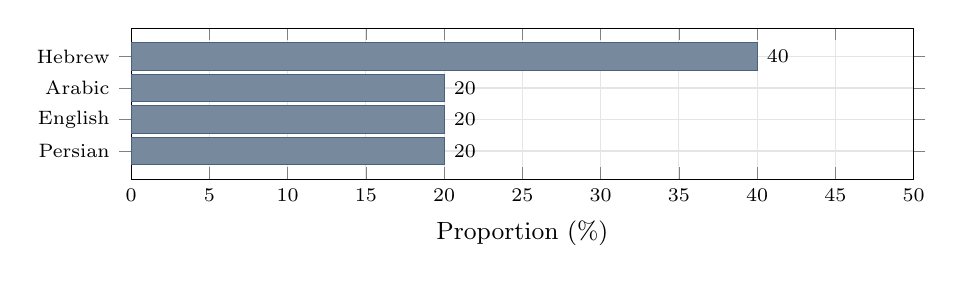
\begin{tikzpicture}
\begin{axis}[
    xbar,
    bar width=10pt,
    xlabel={Proportion (\%)},
    symbolic y coords={Persian, English, Arabic, Hebrew},
    ytick=data,
    xmin=0, xmax=50,
    nodes near coords,
    nodes near coords align={horizontal},
    every node near coord/.append style={font=\scriptsize\bfseries},
    width=0.95\columnwidth,
    height=3.5cm,
    bar shift=0pt,
    enlarge y limits=0.3,
    xmajorgrids=true,
]
\addplot[fill=accent!60, draw=accent!80] coordinates {(40,Hebrew) (20,Arabic) (20,English) (20,Persian)};
\end{axis}
\end{tikzpicture}
\caption{Pretraining data distribution. Hebrew is overrepresented as the anchor language.}
\label{fig:data_dist}
\end{figure}

Hebrew is intentionally overrepresented to ensure strong anchor-language representations. By ``anchor language,'' we mean a language that receives extra training emphasis so that the model builds especially strong internal representations for it, which may then help related languages through shared structure. Data preprocessing includes MinHash deduplication, perplexity-based quality filtering, and language identification verification.

\subsection{Architecture}

SemiticGPT uses a decoder-only transformer with modern enhancements:

\begin{table}[H]
\centering\small
\begin{tabular}{ll}
\toprule
\textbf{Hyperparameter} & \textbf{Value} \\
\midrule
Parameters & 3.14B \\
Layers & 26 \\
Hidden dimension & 3,072 \\
Attention heads & 24 \\
Head dimension & 128 \\
Vocabulary size & 32,000 \\
Max sequence length & 2,048 \\
Position encoding & RoPE ($\theta$=10,000) \\
Activation & SwiGLU \\
Normalization & RMSNorm ($\epsilon$=1e-6) \\
\bottomrule
\end{tabular}
\caption{SemiticGPT architecture.}
\label{tab:architecture}
\end{table}

\subsection{Pretraining}

Training uses AWS spot instances (L40S 48GB and H100 80GB). Configuration:

\begin{itemize}
    \item \textbf{Optimizer}: AdamW ($\beta_1$=0.9, $\beta_2$=0.95)
    \item \textbf{Learning rate}: 3e-4 peak, cosine decay to 3\%
    \item \textbf{Warmup}: 2,000 steps
    \item \textbf{Batch size}: 512K tokens (via gradient accumulation)
    \item \textbf{Weight decay}: 0.1 \quad \textbf{Gradient clipping}: 1.0
    \item \textbf{Precision}: bfloat16
\end{itemize}

Total cost: approximately \$1,456 using spot instances at 60--70\% discount.

\subsection{Supervised Fine-Tuning (SFT)}
\label{sec:sft}

Supervised fine-tuning (SFT) is the stage after pretraining where the model is trained on labeled examples for specific behaviors or tasks. In this paper, SFT is the mechanism that teaches the pretrained model how to perform sentiment classification and use parallel translation examples more effectively.

We conduct SFT using 36,980 multilingual samples:

\begin{itemize}
    \item \textbf{Sentiment data} (18,980 samples): Binary sentiment classification across all four languages, sourced from native-language datasets (Hebrew: HebEMO; Arabic: HARD; Persian: DeepSentiPers; English: SST-2).
    \item \textbf{Translation data} (18,000 samples): Parallel sentence pairs from OPUS-100 \citep{zhang2020improving}, covering all six language-pair directions.
\end{itemize}

\textbf{Data quality.} After identifying critical data bugs in earlier SFT iterations (Section~\ref{sec:data_lessons}), the final dataset enforces: (1) correct label alignment verified per-dataset, (2) random shuffling before train/eval split, (3) strict separation with no data leakage, and (4) balanced 50/50 class distribution in all evaluation sets.

SFT training: AdamW optimizer, learning rate 2e-5, cosine schedule, 8,000 steps, sequence length 384, bfloat16 precision. Best validation loss: 1.98.

For the cross-lingual transfer experiment (Experiment B), we also train an \textbf{English-only SFT} variant using only the English subset (4,745 samples) with identical hyperparameters for 2,000 steps.

% ============================================================
\section{Experiments and Results}

We evaluate SemiticGPT through three focused experiments designed to answer specific questions about multilingual pretraining efficiency.

\subsection{Evaluation Methodology}

\textbf{Sentiment classification.} We use two complementary methods:
\begin{itemize}
    \item \textbf{Logprob}: Compare log-probabilities of ``positive'' vs ``negative'' completion tokens given the input text and a classification prompt. This avoids generation parsing issues. In simpler terms, instead of asking the model to generate a full answer and then trying to interpret it, we directly measure which label the model considers more likely. This makes the evaluation more stable and less sensitive to formatting quirks. $N$=200 per language.
    \item \textbf{Generative}: The model generates a free-form classification response. Outputs are parsed for sentiment labels. This is closer to how users interact with chat models in practice, but it is also more fragile: a model may understand the task yet still fail to produce an answer in exactly the expected format. $N$=50 per language.
\end{itemize}

All evaluation sets are balanced (50\% positive, 50\% negative), so chance performance is 50\% for logprob and 0\% for generative (where the model must produce a parseable label).

\textbf{Belebele} \citep{bandarkar2023belebele}: 4-way multiple-choice reading comprehension. $N$=100 per language. Chance = 25\%.

\textbf{Cross-lingual retrieval}: Given a sentence in language A, retrieve its translation from 10 candidates in language B using cosine similarity of mean-pooled hidden states. Chance = 10\%. Intuitively, this tests whether the model places sentences with the same meaning close together in its internal representation space, even when they are written in different languages.

\subsection{Experiment A: Multilingual Downstream Evaluation}
\label{sec:exp_a}

We evaluate sentiment classification at three model stages: base (pretrained only), English-only SFT, and multilingual SFT. This three-stage comparison is designed to separate three distinct capabilities: what the model learns from pretraining alone, what it gains from task training in English only, and what additional benefit comes from exposing it to task data in all target languages.

\begin{table}[H]
\centering\small
\begin{tabular}{lccccc}
\toprule
\textbf{Stage} & \textbf{HE} & \textbf{AR} & \textbf{FA} & \textbf{EN} \\
\midrule
\multicolumn{5}{l}{\textit{Logprob classification (N=200, chance=50\%)}} \\
Base & 53.0 & 45.0 & 60.5 & 51.5 \\
EN-SFT & 51.5 & 46.5 & 58.5 & 52.0 \\
Multi-SFT & \textbf{84.5} & \textbf{60.5} & \textbf{78.5} & \textbf{73.0} \\
\midrule
\multicolumn{5}{l}{\textit{Generative classification (N=50, chance=0\%)}} \\
Base & 0 & 0 & 0 & 0 \\
EN-SFT & 0 & 0 & 0 & 2 \\
Multi-SFT & \textbf{82} & \textbf{64} & \textbf{74} & \textbf{64} \\
\bottomrule
\end{tabular}
\caption{Sentiment accuracy (\%) across three model stages. Multilingual SFT produces large gains across all languages; English-only SFT does not.}
\label{tab:sentiment}
\end{table}

Key observations:
\begin{enumerate}
    \item \textbf{Base model}: Near chance for logprob (50--60\%), zero for generative. The pretrained model has no task-following ability.
    \item \textbf{English-only SFT}: Negligible improvement on any language including English itself (+0.5pp logprob). The model learns to follow English instructions but this does not transfer to sentiment understanding.
    \item \textbf{Multilingual SFT}: Large gains across all languages. Hebrew improves most (+31.5pp logprob, 82\% generative), consistent with its role as the pretraining anchor language.
\end{enumerate}

\begin{figure}[H]
\centering
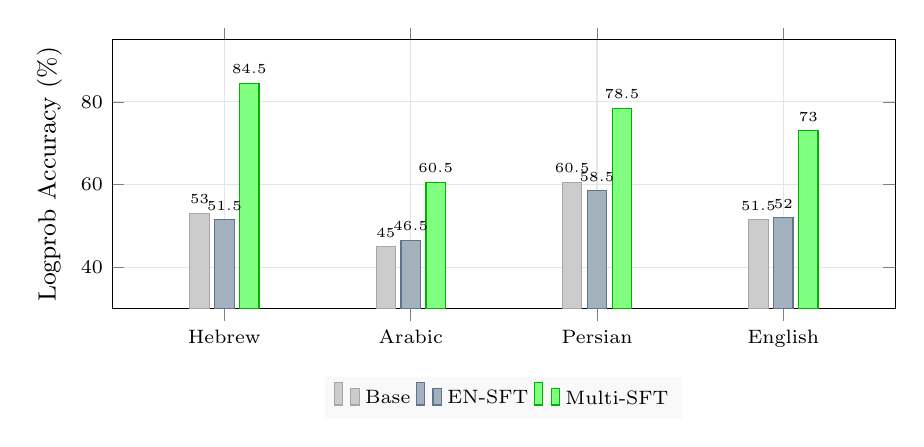
\begin{tikzpicture}
\begin{axis}[
    ybar,
    bar width=7pt,
    ylabel={Logprob Accuracy (\%)},
    symbolic x coords={Hebrew, Arabic, Persian, English},
    xtick=data,
    ymin=30, ymax=95,
    legend style={at={(0.5,-0.25)}, anchor=north, legend columns=3, font=\scriptsize},
    nodes near coords,
    nodes near coords align={vertical},
    every node near coord/.append style={font=\tiny},
    width=0.95\columnwidth,
    height=5cm,
    ymajorgrids=true,
    enlarge x limits=0.2,
]
\addplot[fill=gray!40, draw=gray!70] coordinates {(Hebrew,53.0) (Arabic,45.0) (Persian,60.5) (English,51.5)};
\addplot[fill=accent!40, draw=accent!70] coordinates {(Hebrew,51.5) (Arabic,46.5) (Persian,58.5) (English,52.0)};
\addplot[fill=green!50, draw=green!70!black] coordinates {(Hebrew,84.5) (Arabic,60.5) (Persian,78.5) (English,73.0)};
\legend{Base, EN-SFT, Multi-SFT}
\end{axis}
\end{tikzpicture}
\caption{Sentiment classification across three stages. English-only SFT (blue) produces no meaningful improvement over base (gray). Multilingual SFT (green) yields large gains for all languages.}
\label{fig:sentiment}
\end{figure}

\subsection{Experiment B: Cross-lingual Transfer Analysis}
\label{sec:exp_b}

Experiment B directly tests whether fine-tuning in one language transfers to others. Table~\ref{tab:sentiment} already shows the three-stage progression. The key finding is the \textbf{EN-SFT control}: training on English-only data does not improve non-English sentiment performance, and barely improves English itself.

This contrasts with findings in larger models where English fine-tuning can transfer cross-lingually \citep{conneau2020unsupervised}. At 3B scale with 4.48B pretraining tokens, \textbf{explicit multilingual SFT data is required} for each target language. For practitioners, this means that multilingual pretraining alone is not enough if the goal is downstream performance in low-resource languages: some task-specific examples in those languages are still needed.

\textbf{External baseline context.} As a reference point, XLM-R-Large \citep{conneau2020unsupervised} fine-tuned on XNLI (a 550M parameter encoder model with much larger pretraining data) achieves 79.5\% on English zero-shot sentiment but only 33.5\% on Arabic zero-shot sentiment using our evaluation methodology.\footnote{XLM-R evaluated using zero-shot NLI classification (\texttt{joeddav/xlm-roberta-large-xnli}), N=200 per language. Arabic evaluated on different data (tweet sentiment) due to dataset availability; comparison is approximate.} This suggests that even large multilingual encoder models struggle with zero-shot cross-lingual sentiment transfer, providing context for our 3B decoder model's requirement of explicit multilingual SFT. In other words, the challenge is not unique to our model: even strong multilingual systems can learn shared representations across languages without automatically becoming good at transferring a downstream task across them.

\textbf{Belebele reading comprehension} (Table~\ref{tab:belebele}) shows a similar pattern: all stages perform near chance, confirming that 3B scale is insufficient for abstract reasoning tasks regardless of SFT strategy.

\begin{table}[H]
\centering\small
\begin{tabular}{lcccc}
\toprule
\textbf{Stage} & \textbf{HE} & \textbf{AR} & \textbf{FA} & \textbf{EN} \\
\midrule
Random & 25.0 & 25.0 & 25.0 & 25.0 \\
Base & 26.0 & 22.0 & 19.0 & 19.0 \\
EN-SFT & 26.0 & 23.0 & 20.0 & 20.0 \\
Multi-SFT & 28.0 & 24.0 & 25.0 & 23.0 \\
\bottomrule
\end{tabular}
\caption{Belebele reading comprehension accuracy (\%, N=100). All near chance (25\%), as expected at 3B scale.}
\label{tab:belebele}
\end{table}

\textbf{Cross-lingual embeddings.} Despite limited task transfer, the base model develops strong cross-lingual alignment purely from multilingual pretraining:

\begin{table}[H]
\centering\small
\begin{tabular}{lcc}
\toprule
\textbf{Direction} & \textbf{Base} & \textbf{Multi-SFT} \\
\midrule
EN$\rightarrow$HE & 90\% & 90\% \\
HE$\rightarrow$EN & 90\% & 80\% \\
AR$\rightarrow$EN & 70\% & 50\% \\
AR$\rightarrow$HE & 70\% & 70\% \\
EN$\rightarrow$AR & 50\% & 60\% \\
HE$\rightarrow$AR & 40\% & 60\% \\
FA$\rightarrow$HE & 50\% & 30\% \\
HE$\rightarrow$FA & 40\% & 30\% \\
EN$\rightarrow$FA & 20\% & 20\% \\
AR$\rightarrow$FA & 10\% & 10\% \\
FA$\rightarrow$EN & 10\% & 10\% \\
FA$\rightarrow$AR & 10\% & 10\% \\
\midrule
\textbf{Average} & \textbf{45.8\%} & \textbf{43.3\%} \\
\bottomrule
\end{tabular}
\caption{Cross-lingual retrieval accuracy (10-way, chance=10\%). Strong EN$\leftrightarrow$HE alignment emerges from pretraining alone.}
\label{tab:embeddings}
\end{table}

English$\leftrightarrow$Hebrew achieves 90\% retrieval (9$\times$ chance), and Arabic shows meaningful alignment with both English and Hebrew. Persian shows weak connectivity, consistent with its typological distance from the Semitic family.

Notably, multilingual SFT improves downstream sentiment while slightly reducing average retrieval accuracy (45.8\%$\rightarrow$43.3\%). This suggests that downstream task adaptation may trade off against some alignment properties of the pretrained representation space---the model becomes better at following task instructions but slightly less balanced as a general-purpose cross-lingual encoder. A useful intuition is that fine-tuning can make the model better at one job while making its internal representations slightly less general-purpose. Better task accuracy does not always mean better universal embeddings.

\begin{figure}[H]
\centering
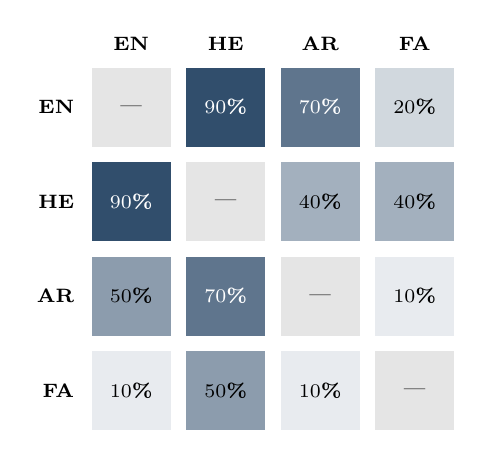
\begin{tikzpicture}
\def\data{{
    {0,90,70,20},
    {90,0,40,40},
    {50,70,0,10},
    {10,50,10,0}}};
\def\langs{{"EN","HE","AR","FA"}}
\foreach \row in {0,...,3} {
    \foreach \col in {0,...,3} {
        \ifnum\row=\col
            \fill[black!10] (\col*1.2, -\row*1.2) rectangle (\col*1.2+1.0, -\row*1.2+1.0);
            \node[font=\scriptsize] at (\col*1.2+0.5, -\row*1.2+0.5) {---};
        \else
            \pgfmathsetmacro{\val}{\data[\row][\col]}
            \fill[accent!\val] (\col*1.2, -\row*1.2) rectangle (\col*1.2+1.0, -\row*1.2+1.0);
            \pgfmathsetmacro{\textcol}{ifthenelse(\val>50, "white", "black")}
            \node[font=\scriptsize\bfseries, text=\textcol] at (\col*1.2+0.5, -\row*1.2+0.5) {\pgfmathprintnumber[fixed,precision=0]{\val}\%};
        \fi
    }
}
\foreach \col in {0,...,3} {
    \pgfmathsetmacro{\lbl}{\langs[\col]}
    \node[font=\scriptsize\bfseries, above] at (\col*1.2+0.5, 1.1) {\lbl};
}
\foreach \row in {0,...,3} {
    \pgfmathsetmacro{\lbl}{\langs[\row]}
    \node[font=\scriptsize\bfseries, left] at (-0.1, -\row*1.2+0.5) {\lbl};
}
\end{tikzpicture}
\caption{Cross-lingual retrieval heatmap (base model, 10-way, chance=10\%). Darker = stronger alignment. EN$\leftrightarrow$HE alignment is strongest.}
\label{fig:heatmap}
\end{figure}

\subsection{Experiment C: Tokenizer Ablation}
\label{sec:exp_c}

We compare our custom 32K tokenizer against two baselines of identical vocabulary size: Llama-2 (English-centric) and HebrewGPT-1B (Hebrew-centric). All three use 32K BPE vocabularies. Tokenizer efficiency matters because every extra token consumes context window space and training compute. A language that is split into many small pieces is effectively harder and more expensive for the model to process.

\subsubsection{Vocabulary Composition}

\begin{table}[H]
\centering\small
\begin{tabular}{lccc}
\toprule
\textbf{Script} & \textbf{Ours} & \textbf{Llama-2} & \textbf{HebrewGPT} \\
\midrule
Arabic script & 46.7\% & 0.2\% & 0.4\% \\
Hebrew script & 27.8\% & 0.1\% & 72.2\% \\
Latin script & 24.3\% & 80.9\% & 7.0\% \\
Other & 1.2\% & 18.8\% & 20.4\% \\
\bottomrule
\end{tabular}
\caption{Vocabulary composition by script. Our tokenizer balances Arabic (covering both Arabic and Persian), Hebrew, and Latin. Llama-2 is 81\% Latin; HebrewGPT is 72\% Hebrew.}
\label{tab:vocab_comp}
\end{table}

\subsubsection{Encoding Efficiency}

\begin{table}[H]
\centering\small
\begin{tabular}{lcccr}
\toprule
\textbf{Lang} & \textbf{Ours} & \textbf{Llama-2} & \textbf{HebrewGPT} & \textbf{$\Delta$ vs Llama} \\
\midrule
\multicolumn{5}{l}{\textit{Fertility (tokens per word, lower is better)}} \\
\multicolumn{5}{l}{\scriptsize A lower fertility means the tokenizer represents each word using fewer pieces.} \\
EN & 1.54 & 1.51 & 2.42 & $-$2.0\% \\
HE & \textbf{1.34} & 3.91 & 1.26 & \textbf{+65.7\%} \\
AR & \textbf{2.22} & 4.36 & 4.15 & \textbf{+49.1\%} \\
FA & \textbf{1.52} & 4.88 & 4.51 & \textbf{+68.8\%} \\
\midrule
\multicolumn{5}{l}{\textit{Bytes per token (higher is better)}} \\
\multicolumn{5}{l}{\scriptsize Higher bytes per token means each token carries more text on average.} \\
EN & 3.71 & 3.79 & 2.37 & $-$2.1\% \\
HE & \textbf{5.12} & 1.76 & 5.48 & \textbf{+191\%} \\
AR & \textbf{3.48} & 1.77 & 1.86 & \textbf{+97\%} \\
FA & \textbf{5.72} & 1.78 & 1.93 & \textbf{+221\%} \\
\bottomrule
\end{tabular}
\caption{Tokenizer efficiency comparison. Our tokenizer matches Llama-2 on English while using 49--69\% fewer tokens for Hebrew, Arabic, and Persian. HebrewGPT excels on Hebrew but fragments Arabic/Persian.}
\label{tab:tokenizer}
\end{table}

\begin{figure}[H]
\centering
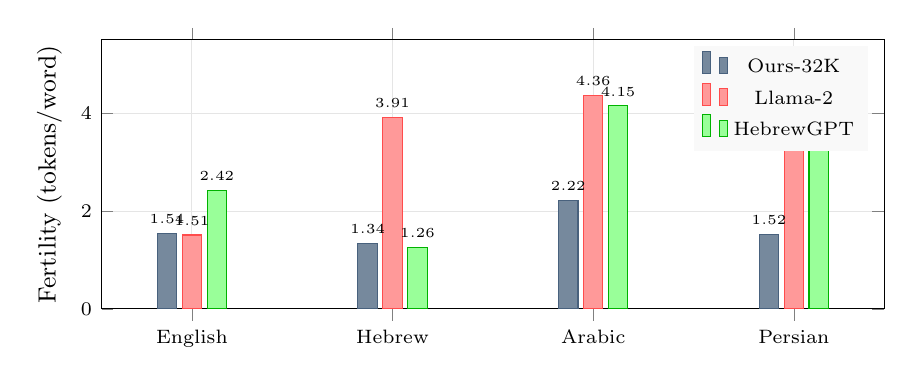
\begin{tikzpicture}
\begin{axis}[
    ybar,
    bar width=7pt,
    ylabel={Fertility (tokens/word)},
    symbolic x coords={English, Hebrew, Arabic, Persian},
    xtick=data,
    ymin=0, ymax=5.5,
    legend style={at={(0.98,0.98)}, anchor=north east, legend columns=1, font=\scriptsize},
    width=0.95\columnwidth,
    height=5cm,
    ymajorgrids=true,
    enlarge x limits=0.15,
    nodes near coords,
    nodes near coords align={vertical},
    every node near coord/.append style={font=\tiny},
]
\addplot[fill=accent!60, draw=accent!80] coordinates {(English,1.54) (Hebrew,1.34) (Arabic,2.22) (Persian,1.52)};
\addplot[fill=red!40, draw=red!70] coordinates {(English,1.51) (Hebrew,3.91) (Arabic,4.36) (Persian,4.88)};
\addplot[fill=green!40, draw=green!70!black] coordinates {(English,2.42) (Hebrew,1.26) (Arabic,4.15) (Persian,4.51)};
\legend{Ours-32K, Llama-2, HebrewGPT}
\end{axis}
\end{tikzpicture}
\caption{Tokenizer fertility comparison. Lower is better. Our tokenizer achieves near-parity with Llama-2 on English while dramatically reducing fragmentation for Hebrew, Arabic, and Persian.}
\label{fig:fertility}
\end{figure}

Key findings:
\begin{enumerate}
    \item \textbf{No English penalty}: Our tokenizer matches Llama-2 on English (1.54 vs 1.51 tokens/word), a common concern when balancing non-Latin scripts.
    \item \textbf{Massive efficiency for target languages}: Hebrew uses 66\% fewer tokens, Arabic 49\% fewer, Persian 69\% fewer than Llama-2. This directly translates to longer effective context windows and reduced training cost.
    \item \textbf{Specialization tradeoff}: HebrewGPT-1B slightly outperforms ours on Hebrew (1.26 vs 1.34) but fragments Arabic/Persian as badly as Llama-2. A multilingual tokenizer must balance all target languages.
\end{enumerate}

\subsubsection{Segmentation Examples}

To illustrate the practical impact, consider two examples:

\textbf{Hebrew:} ``habina hamela'khutit meshane et ha'olam'' (Artificial intelligence is changing the world):
\begin{itemize}
    \item \textbf{Ours}: 4 tokens (whole-word segmentation)
    \item \textbf{Llama-2}: 18 tokens (character-level fragmentation)
    \item \textbf{HebrewGPT}: 5 tokens (comparable---Hebrew-optimized)
\end{itemize}

\textbf{Arabic:} ``asimat faransa hia baris'' (The capital of France is Paris):

\begin{itemize}
    \item \textbf{Ours}: 5 tokens (whole-word segmentation)
    \item \textbf{Llama-2}: 22 tokens (character-level fragmentation)
    \item \textbf{HebrewGPT}: 19 tokens (character-level fragmentation)
\end{itemize}

Our tokenizer captures whole Arabic words as single tokens, while the baselines fragment at the character level---a 4.4$\times$ efficiency difference on this sentence.

% ============================================================
\section{Analysis and Discussion}

\subsection{The Multilingual SFT Requirement}

The most important finding is the sharp contrast between English-only and multilingual SFT (Figure~\ref{fig:sentiment}). At 3B scale with 4.48B pretraining tokens, the model does not develop sufficient cross-lingual task transfer from English fine-tuning alone. This differs from observations in much larger models (175B+ parameters) where English fine-tuning shows some cross-lingual generalization.

The key negative result is not merely that English-only SFT helps \emph{less}, but that it helps \emph{almost not at all}---despite measurable cross-lingual representational alignment from pretraining (90\% EN$\leftrightarrow$HE retrieval). The pretrained model ``knows'' these languages are related at the representation level, but cannot use that knowledge for tasks without explicit multilingual fine-tuning. Put simply, the model learns that related languages belong in a shared semantic space, but it still needs explicit examples in those languages to learn how to apply that knowledge to a specific task.

\textbf{Why does this matter for practitioners?} Researchers building models for low-resource languages cannot rely on cheap English-only SFT and hope for cross-lingual transfer. They must invest in multilingual SFT data for each target language---but relatively small amounts suffice (our SFT uses only 36,980 total samples).

\subsection{Representation vs.\ Task Transfer}

An intriguing asymmetry: the base model develops strong cross-lingual \emph{representations} (90\% EN$\leftrightarrow$HE retrieval) but cannot leverage them for \emph{tasks} without explicit SFT. Multilingual pretraining builds a shared semantic space, but task-specific fine-tuning is the key that unlocks it. An analogy: pretraining builds a multilingual map, while fine-tuning teaches the model which route to take for a particular task.

\subsection{Hebrew as Anchor Language}

Hebrew shows the strongest results across all experiments: highest sentiment accuracy (84.5\%), strongest embedding alignment with English, and best tokenizer coverage. This is consistent with Hebrew receiving 40\% of pretraining data. Whether anchor overrepresentation produces \emph{disproportionate} returns (beyond the linear expectation from more data) remains an open question that would require controlled ablation (e.g., 40\% vs 25\% Hebrew) to answer.

\subsection{Persian Isolation}

Persian consistently shows weak cross-lingual connectivity despite sharing Arabic script. In our retrieval experiment, Persian achieves only 10--30\% accuracy with other languages, compared to 40--90\% for the Hebrew-Arabic-English triad. Our results are consistent with linguistic family membership being a stronger predictor of transfer than script similarity in this setup, though we cannot fully disentangle this from Persian's 20\% pretraining share vs Hebrew's 40\%.

\subsection{Data Quality Lessons}
\label{sec:data_lessons}

During development, we discovered critical data bugs that invalidated earlier results. These errors are worth documenting because they changed the conclusions of earlier experiments and illustrate how easily low-resource evaluation pipelines can produce misleading results.

\begin{enumerate}
    \item \textbf{Hebrew label inversion}: The dataset's label encoding (0=positive) was opposite to our assumption (0=negative), causing the model to learn inverted sentiment.
    \item \textbf{Arabic sorting artifact}: The dataset was sorted by label before splitting, causing the training set to contain only negative examples.
    \item \textbf{Translation data quality}: Early iterations used 50 hardcoded sentence pairs instead of real parallel data.
\end{enumerate}

\textbf{Lesson}: Automated data pipeline audits---checking label distributions, train/eval overlap, and sample diversity---should be mandatory before any training run. We now enforce 50/50 class balance and verify shuffle randomness in all evaluation sets.

\subsection{Cost Analysis}

\begin{table}[H]
\centering\small
\begin{tabular}{lcr}
\toprule
\textbf{Component} & \textbf{GPU-hours} & \textbf{Cost} \\
\midrule
Proxy experiments (32 runs) & 16 & \$12 \\
Pretraining (4.48B tokens) & 380 & \$1,380 \\
SFT (36,980 samples) & 4 & \$14 \\
Evaluation (all experiments) & 8 & \$30 \\
\midrule
\textbf{Total} & \textbf{408} & \textbf{$\sim$\$1,436} \\
\bottomrule
\end{tabular}
\caption{Cost breakdown. All compute on AWS spot instances (60--70\% discount).}
\label{tab:cost}
\end{table}

% ============================================================
\section{Practitioner's Guide}
\label{sec:guide}

Based on our experience, we provide recommendations for researchers building similar multilingual models. The recommendations below are not general laws; they are practical lessons distilled from the experiments and failure cases reported in this paper.

\subsection{Language Cluster Selection}

\begin{itemize}
    \item Our results are consistent with \textbf{linguistic family membership} being a stronger predictor of transfer than script similarity. Include a typologically distant language as a control condition.
\end{itemize}

\subsection{Tokenizer Design}

\begin{itemize}
    \item Train a \textbf{custom BPE tokenizer} on equally-weighted samples of all target languages. Do \emph{not} reuse an English-centric tokenizer---it wastes 49--69\% of tokens on non-Latin scripts.
    \item \textbf{32K vocabulary} is sufficient for 4--6 languages. Target fertility $\leq$2.0 tokens/word for all languages.
    \item The English efficiency penalty from balancing is minimal ($-$2\% in our case).
\end{itemize}

\subsection{Pretraining}

\begin{itemize}
    \item \textbf{Anchor overrepresentation} (30--40\% for primary language) appears beneficial but is not ablated in this work.
    \item Use \textbf{spot instances with checkpointing} every 30 minutes for cost efficiency.
    \item \textbf{bfloat16}: We observed no degradation in our setup compared to float32 in preliminary experiments.
    \item Validate recipe at proxy scale (100--200M parameters) before full commitment.
\end{itemize}

\subsection{Supervised Fine-Tuning}

\begin{itemize}
    \item \textbf{Include all target languages} in SFT data. In our experiments, English-only SFT was insufficient at 3B scale.
    \item \textbf{Native-language data $>$ machine-translated data}. We found translated Alpaca produces weaker results than native-language datasets.
    \item \textbf{Audit data pipelines} before training: verify label encoding, check for sorting artifacts, confirm train/eval separation.
    \item 37K samples with 8K steps was sufficient for our model.
\end{itemize}

\subsection{Evaluation}

\begin{itemize}
    \item Use \textbf{logprob-based evaluation} for classification tasks---it avoids prompt/parsing issues that plague generative evaluation.
    \item \textbf{Always report chance level} for each metric.
    \item Cross-lingual retrieval requires \textbf{no labeled data} and reveals representational quality.
    \item Expect \textbf{near-chance results on reasoning benchmarks} (Belebele, MMLU) at 3B scale. This is not a failure---it calibrates expectations.
\end{itemize}

\begin{table}[H]
\centering\scriptsize
\begin{tabular}{lp{4cm}}
\toprule
\textbf{Decision} & \textbf{Recommendation} \\
\midrule
Language selection & Linguistic family $>$ script (in our setup) \\
Tokenizer & Custom BPE, 32K vocab, balanced \\
Anchor language & Over-represent at 30--40\% \\
Recipe validation & 20--50 proxy experiments first \\
Optimizer & AdamW ($\beta_2$=0.95) \\
Precision & bfloat16 \\
SFT data & All target languages required \\
SFT source & Native-language $>$ translated \\
Data quality & Audit labels, splits, balance \\
Evaluation & Logprob $>$ generative for classification \\
Compute & Cloud spot instances + checkpointing \\
\bottomrule
\end{tabular}
\caption{Recipe summary for building multilingual models from scratch.}
\label{tab:recipe}
\end{table}

% ============================================================
\section{Limitations}
\label{sec:limitations}

\begin{itemize}
    \item \textbf{Single-run results}: All experiments are single-run without confidence intervals. Effects under 5 percentage points may not be statistically significant. Key findings (e.g., 84.5\% vs 51.5\% sentiment) are large enough to be meaningful.
    \item \textbf{Small evaluation sets}: 200 samples for logprob, 50 for generative, 100 for Belebele. Sufficient for detecting large effects but not small ones.
    \item \textbf{Limited external baselines}: We provide a partial XLM-R comparison (Section~\ref{sec:exp_b}), but a full apples-to-apples comparison on identical datasets against mBERT, XLM-R, and multilingual instruction models would better contextualize our results.
    \item \textbf{Scale}: At 3B parameters, the model is below thresholds for complex reasoning. Findings about transfer requirements may not hold at larger scales where English-only SFT \emph{does} transfer.
    \item \textbf{Confounded variables}: Hebrew receives 40\% of pretraining data vs Persian's 20\%. Persian's weak transfer may partly reflect data quantity rather than purely typological distance.
    \item \textbf{Anchor ablation}: We do not ablate the effect of anchor overrepresentation (e.g., 40\% Hebrew vs 25\% balanced).
    \item \textbf{Generalizability}: Our recipe is demonstrated on one language cluster. Whether the same principles apply to other families (Turkic, Bantu, Dravidian) is an empirical question.
\end{itemize}

% ============================================================
\section{Conclusion}

We present SemiticGPT, a 3.14B parameter multilingual model covering Hebrew, Arabic, Persian, and English, trained from scratch for under \$1,500. Our three experiments establish that:

\begin{enumerate}
    \item \textbf{Multilingual SFT is required in this setting}: English-only fine-tuning is insufficient for non-English downstream tasks at 3B scale. Explicit multilingual SFT data unlocks the cross-lingual representations built during pretraining.
    \item \textbf{Custom tokenizers eliminate waste}: A balanced tokenizer uses 49--69\% fewer tokens than English-centric alternatives for target languages, with negligible English penalty.
    \item \textbf{Cross-lingual representations emerge before task transfer}: The model builds strong cross-lingual embeddings (90\% EN$\leftrightarrow$HE retrieval) from pretraining alone, but task-specific multilingual SFT is needed to leverage them for downstream performance.
\end{enumerate}

More broadly, our results suggest that for smaller multilingual models, shared language representations can emerge during pretraining, but usable cross-lingual task performance still depends on explicit multilingual supervision. We release all code, data, and model weights to support reproducible research and provide a practitioner's guide for researchers targeting other under-resourced language families.

\textbf{Future work.} Scaling to 7B+ parameters to test whether cross-lingual SFT transfer emerges at larger scale; adding more Semitic languages (Amharic, Tigrinya); ablating anchor language overrepresentation; and improving Arabic SFT with higher-quality native datasets.

% ============================================================
\section{Reproducibility}

All artifacts are available at \url{https://github.com/fatherRonnen/semitic-gpt}:

\begin{table}[H]
\centering\scriptsize
\begin{tabular}{lll}
\toprule
\textbf{Section} & \textbf{Repo Path} & \textbf{Contents} \\
\midrule
Tokenizer (\S3.1) & \texttt{tokenizer/} & Config, training script, fertility \\
Data (\S3.2) & \texttt{data/} & Collection scripts, manifests \\
Proxy (\S2) & \texttt{proxy/} & 32 configs, results \\
Pretraining (\S3.4) & \texttt{pretrain/} & Scripts, hyperparams, logs \\
SFT (\S3.5) & \texttt{sft/} & Configs, scripts, v4 pipeline \\
Experiments (\S4) & \texttt{eval/} & Scripts, prompts, results \\
\bottomrule
\end{tabular}
\caption{Paper-to-repository mapping.}
\label{tab:reproducibility}
\end{table}

Model weights (base: 6.1GB, SFT: 6.3GB) and tokenizer are available on HuggingFace at \url{https://huggingface.co/Slasky/SemiticGPT-3B}.

% ============================================================
\bibliographystyle{plainnat}
\begin{thebibliography}{99}

\bibitem[Antoun et al.(2021)]{antoun2021aragpt2}
W.~Antoun, F.~Baly, and H.~Hajj.
\newblock AraGPT2: Pre-trained transformer for Arabic language generation.
\newblock In \emph{Proc. WANLP}, 2021.

\bibitem[Bandarkar et al.(2023)]{bandarkar2023belebele}
L.~Bandarkar et al.
\newblock The Belebele benchmark: a parallel reading comprehension dataset in 122 language variants.
\newblock \emph{arXiv:2308.16884}, 2023.

\bibitem[Conneau et al.(2020)]{conneau2020unsupervised}
A.~Conneau, K.~Khandelwal, N.~Goyal, et al.
\newblock Unsupervised cross-lingual representation learning at scale.
\newblock In \emph{Proc. ACL}, 2020.

\bibitem[Joshi et al.(2020)]{joshi2020state}
P.~Joshi, S.~Santy, A.~Buber, et al.
\newblock The state and fate of linguistic diversity and inclusion in the NLP world.
\newblock In \emph{Proc. ACL}, 2020.

\bibitem[Koub\^{a}a and Ammar(2024)]{koubaa2024arabiangpt}
A.~Koub\^{a}a and A.~Ammar.
\newblock ArabianGPT: Native Arabic GPT-based large language model.
\newblock \emph{arXiv:2402.15313}, 2024.

\bibitem[Marco-LLM(2024)]{marco2024}
Marco-LLM Team.
\newblock Marco-LLM: Bridging languages via massive multilingual training for cross-lingual enhancement.
\newblock \emph{arXiv:2412.04003}, 2024.

\bibitem[Rivas et al.(2024)]{rivas2024hearbert}
A.~Rivas et al.
\newblock HeArBERT: A bilingual model for Arabic-Hebrew translation using transliteration.
\newblock \emph{arXiv:2402.16065}, 2024.

\bibitem[Sengupta et al.(2023)]{sengupta2023jais}
N.~Sengupta et al.
\newblock Jais and Jais-chat: Arabic-centric foundation and instruction-tuned open generative large language models.
\newblock \emph{arXiv:2308.16149}, 2023.

\bibitem[SmolLM3(2025)]{allal2025smollm3}
L.B.~Allal et al.
\newblock SmolLM3: The complete blueprint of a state-of-the-art 3B parameter LLM.
\newblock HuggingFace Technical Report, 2025.

\bibitem[Karpathy(2026)]{karpathy2026autoresearch}
A.~Karpathy.
\newblock autoresearch: Autonomous AI-driven ML experimentation.
\newblock GitHub repository, 2026.

\bibitem[Slasky(2026)]{slasky2026hebrew}
R.~Slasky.
\newblock Autonomous AI-driven Hebrew language model optimization: From random search to optimizer-architecture co-discovery.
\newblock Independent research report, 2026.

\bibitem[Zhang et al.(2020)]{zhang2020improving}
B.~Zhang, P.~Williams, I.~Titov, and R.~Sennrich.
\newblock Improving massively multilingual neural machine translation and zero-shot translation.
\newblock In \emph{Proc. ACL}, 2020.

\end{thebibliography}

\end{document}
